\documentclass[11pt]{article}
\usepackage{amsmath, amssymb}
\usepackage{geometry}
\geometry{margin=1in}
\usepackage{fancyhdr}
\usepackage{lastpage}
\usepackage{parskip} % Better paragraph spacing
\usepackage{titlesec} % Better section formatting
\usepackage{graphicx}
\usepackage{float}
\usepackage[most]{tcolorbox}
\usepackage{lmodern}
\usepackage{caption}

% Define commands for reusable content
\newcommand{\coursename}{CS-401 Applied Data Analysis}
\newcommand{\lecturenum}{03}
\newcommand{\lecturedate}{\today}
\newcommand{\professor}{Maria Brbic}

% Configure section spacing
\titlespacing*{\section}{0pt}{2ex plus 1ex minus .2ex}{1.5ex plus .2ex}
% Header / Footer
\pagestyle{fancy}
\fancyhf{}
\fancyhead[L]{\coursename}
\fancyhead[R]{Lecture \lecturenum}
\fancyfoot[L]{EPFL - Computer Science}
\fancyfoot[C]{Author: Jonathan Dutoit}
\fancyfoot[R]{Page \thepage\ of \pageref{LastPage}}

\begin{document}

\begin{center}
  {\large EPFL - Computer Science} \\[0.5em]
  {\Large \textbf{\coursename}} \\[0.5em]
  {\large Lecture \lecturenum\ --- \lecturedate} \\[0.5em]
  {\large Author: Jonathan Dutoit} \\[0.5em]
  {\large Professor: \professor} \\[0.5em]
\end{center}

\vspace{2cm}

\begin{center}
  {\LARGE \textbf{Visualizing Data}}
\end{center}

\vspace{1cm}

\section*{Uses for data visualization}

\textbf{Flow:} \textcolor{blue}{Ask} an interesting question $\Rightarrow$ \textcolor{blue}{Get} the data $\Rightarrow$  \textcolor{blue}{Explore} the data $\Rightarrow$  \textcolor{blue}{Model} the data $\Rightarrow$  \textcolor{blue}{Communicate} and \textcolor{blue}{visualize} the results. 

\textcolor{purple}{Analysis}: Support reasoning about information
\begin{itemize}
	\item Finding relationships
	\item Discover structure
	\item Quantifying values and influences
	\item Should be part of the data analysis cycle
\end{itemize}

\textcolor{blue}{Communication}: Inform and persuade other
\begin{itemize}
	\item Capture attention, engage
	\item Tell a story visually
	\item Can focus on certain aspects and omit other
\end{itemize}

\textcolor{green}{Decision making}: Make it easier to evaluate potential courses of action

\section*{Static vs interactive visualization}

\textbf{Static viz}: Great for data exploration, developed throughout the last few centuries...

\textbf{Interactive viz}: More and more common when delivering results (and also during exploration). New frameworks are the key enabler.

In this course we will focus on \textbf{static visualisation}.

There's a dedicated course: COM-480 "Data Visualization"

\newpage 

\section*{Today's lecture}

\begin{itemize}
	\item Part 1: Navigating the chart landscape
	\item Part 2: Principles and best practices
	\item Part 3: A (small) selection of use cases for data visualization
\end{itemize}

\section*{Part 1: Navigating the chart landscape}

% Quick centered image
\begin{figure}[H]
    \centering
    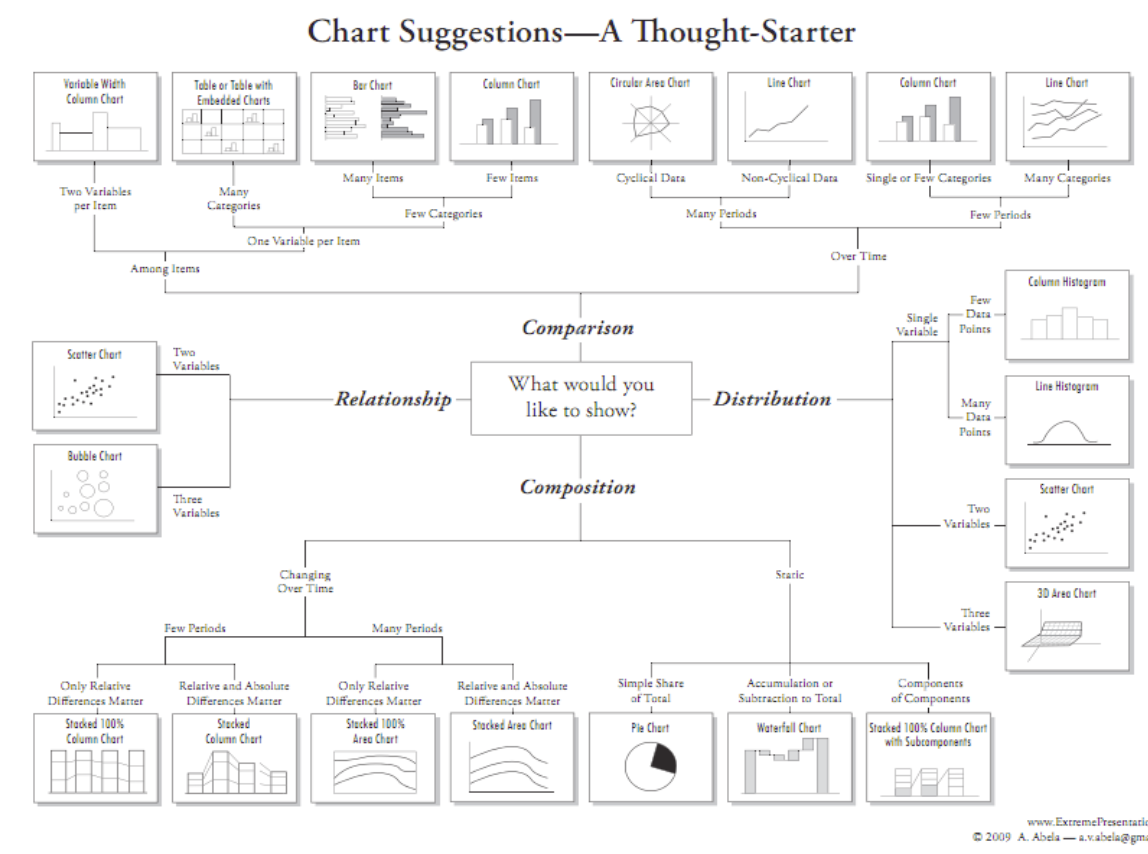
\includegraphics[width=1\textwidth]{chart-selection}
    \label{fig:LABEL}
\end{figure}

\begin{itemize}
      \item \textbf{\textcolor{red}{One variable}}
	\begin{itemize}
		\item \textcolor{red}{Histograms} can tell you a lot about a single variable, discrete or continuous. Easy to recognize skewed distributions! Very powerful data visualization for studying data distribution.
			% Quick centered image
			\begin{figure}[H]
			    \centering
			    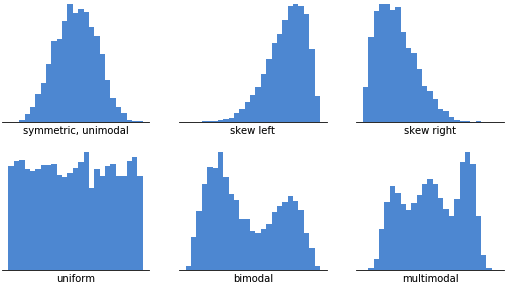
\includegraphics[width=0.6\textwidth]{histograms}
			    \label{fig:LABEL}
			\end{figure}
		\item \textcolor{red}{Box plots} is a method for demonstrating graphically the locality, spread and skewness groups of numerical data through their quartiles. You can see from the Median is the data is normalized or skewed distributed. 
			% Quick centered image
			\begin{figure}[H]
			    \centering
			    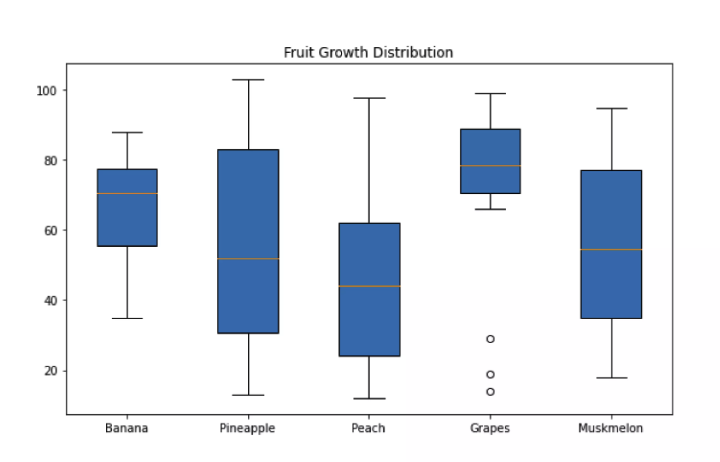
\includegraphics[width=0.6\textwidth]{boxplot}
			    \label{fig:LABEL}
			\end{figure}
	\end{itemize}
     \item \textbf{\textcolor{red}{Two variables}}
	     \begin{itemize}
		     \item \textcolor{red}{Scatter plots} quickly expose the relationships between two variables, often exposing correlation between variables. It's useful when there isn't too many data points. If there are two many data points, some solutions are 2D histograms (\textcolor{blue}{a.k.a heatmap}) 
			     % Quick centered image
			     \begin{figure}[H]
			         \centering
			         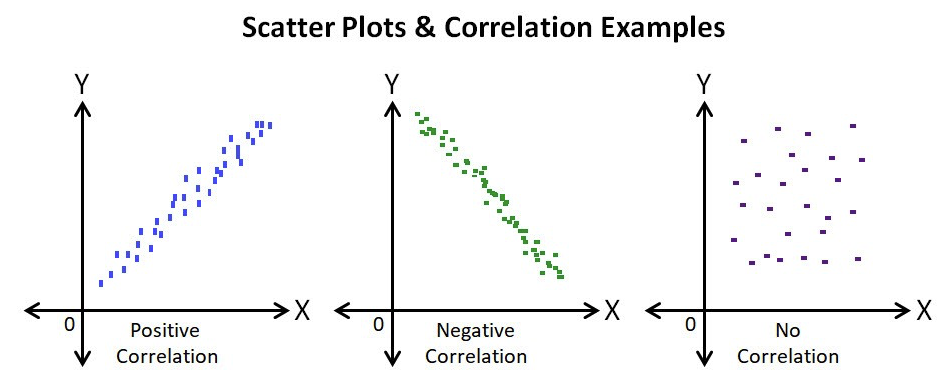
\includegraphics[width=0.6\textwidth]{scatterplot}
			         \label{fig:LABEL}
			     \end{figure}
			     % Quick centered image
			     \begin{figure}[H]
			         \centering
			         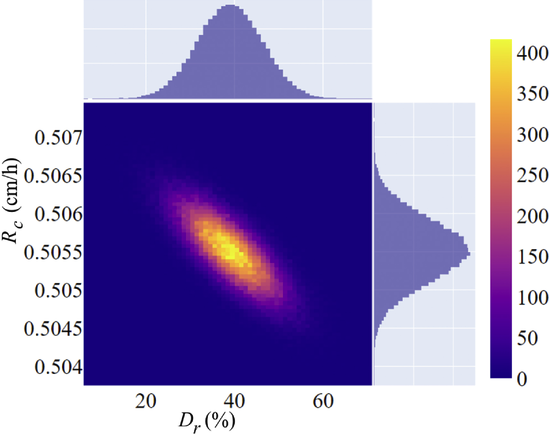
\includegraphics[width=0.5\textwidth]{2dhistogram}
			         \label{fig:LABEL}
			     \end{figure}
			\item \textcolor{red}{Line plots} are useful if the relationship is functional (for instance, after binning and aggregating). For instance, days in the x-axis and stock price in the y-axis.
				% Quick centered image
				\begin{figure}[H]
				    \centering
				    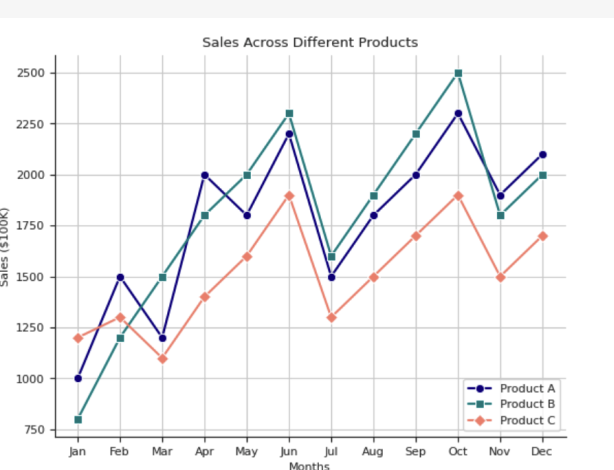
\includegraphics[width=0.5\textwidth]{lineplot}
				    \label{fig:LABEL}
				\end{figure}
	     \end{itemize}
      \item \textcolor{red}{\textbf{$>$ 2 variables}}
	     \begin{itemize}
	     	\item \textcolor{red}{Scatter plot matrix}
			% Quick centered image
			\begin{figure}[H]
			    \centering
			    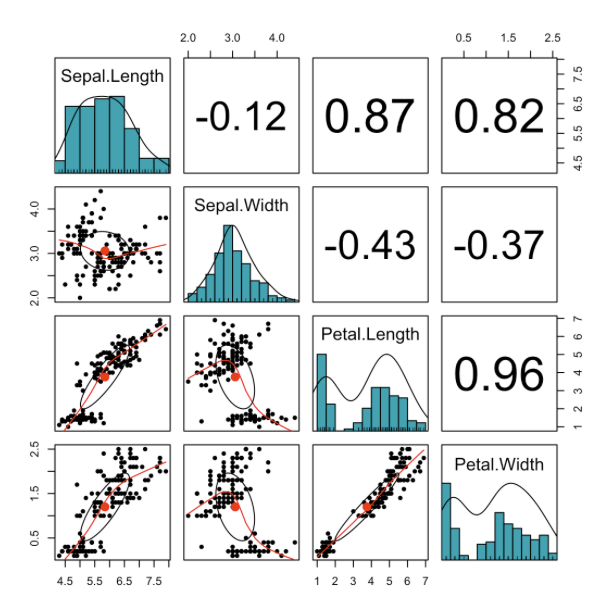
\includegraphics[width=0.5\textwidth]{scatterplotmatrix}
			    \label{fig:LABEL}
			\end{figure}
		\item \textcolor{red}{Stacked plots} often used with many variables: stack index, height, color, etc. Often color variables are categorical, height variables are continuous, stack can be variable and etc. 
			% Quick centered image
			\begin{figure}[H]
			    \centering
			    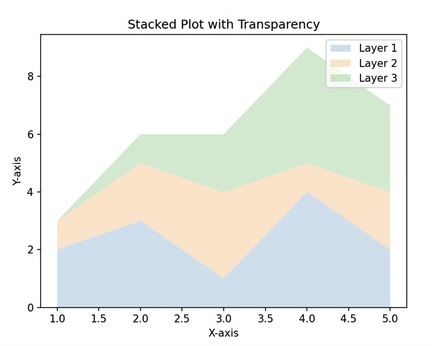
\includegraphics[width=0.5\textwidth]{stackedplot}
			    \label{fig:LABEL}
			\end{figure}
	     \end{itemize}
\end{itemize}

\begin{tcolorbox}[
  colback=gray!15,     % background color
  colframe=black!50,    % border color
  boxrule=1pt,       % border thickness
  arc=3mm,             % rounded corners
  left=4mm, right=4mm, top=2mm, bottom=2mm % padding
]
\textbf{Note}

\vspace{0.3cm}

Use the space wisely when you do data visualization to convey useful information rather than redundant information.
\end{tcolorbox}


\section*{Dimensionally reduction}

\begin{itemize}
	\item For example, \textbf{PCA}: allows visualization of high-dimensional continuous data in 2D using principal components
	\item The principal components are the strongest (highest variation) dimensions in the dataset, and are orthogonal.
\end{itemize}

% Quick centered image
\begin{figure}[H]
    \centering
    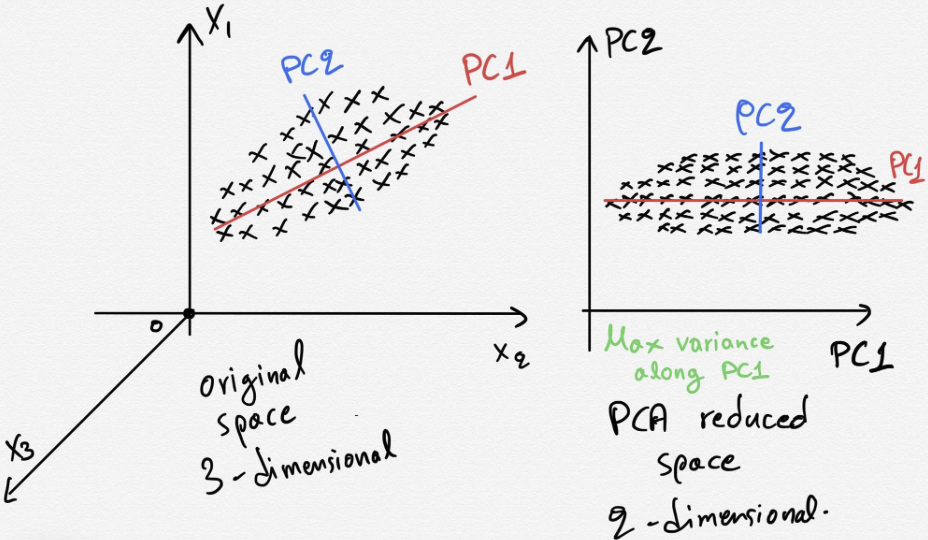
\includegraphics[width=0.6\textwidth]{PCA}
    \label{fig:LABEL}
\end{figure}
\section*{Important example: one dataset, visualized 25 ways}

http://flowingdata.com/2017/01/24/one-dataset-visualized-25-ways


"You must help the data focus and get to the point. Otherwise, it just ends up rambling about what it had for breakfast this morning and how the coffee was not hot enough.”

% Quick centered image
\begin{figure}[H]
    \centering
    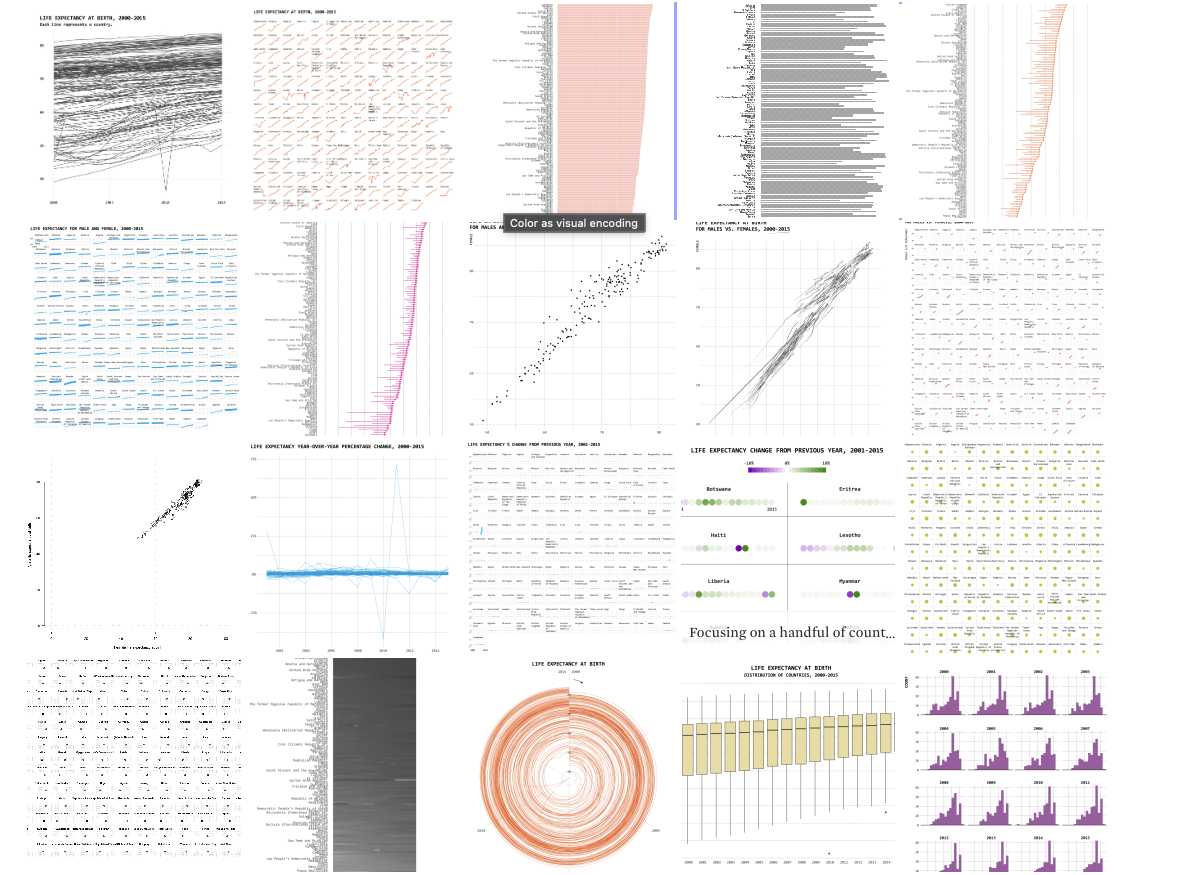
\includegraphics[width=1\textwidth]{example25visua}
    \label{fig:LABEL}
\end{figure}
\newpage

\section*{Part 2: Principles and best practices}

\textcolor{red}{\textbf{Perception of magnitudes}}: some differences are difficult to see with little time. 

\textcolor{red}{\textbf{Just noticable difference (JND)}}

\begin{itemize}
	\item Weber's law: $\frac{\Delta I}{I} = k$
	\item I: intensity; $\Delta I$: increase from I to notice a difference; k: constant
	\item Most continuous variations in stimuli are perceived in discrete (multiplicative) steps
\end{itemize}

As humans, we are most likely to underestimate comparisons between areas/surfaces

% Quick centered image
\begin{figure}[H]
    \centering
    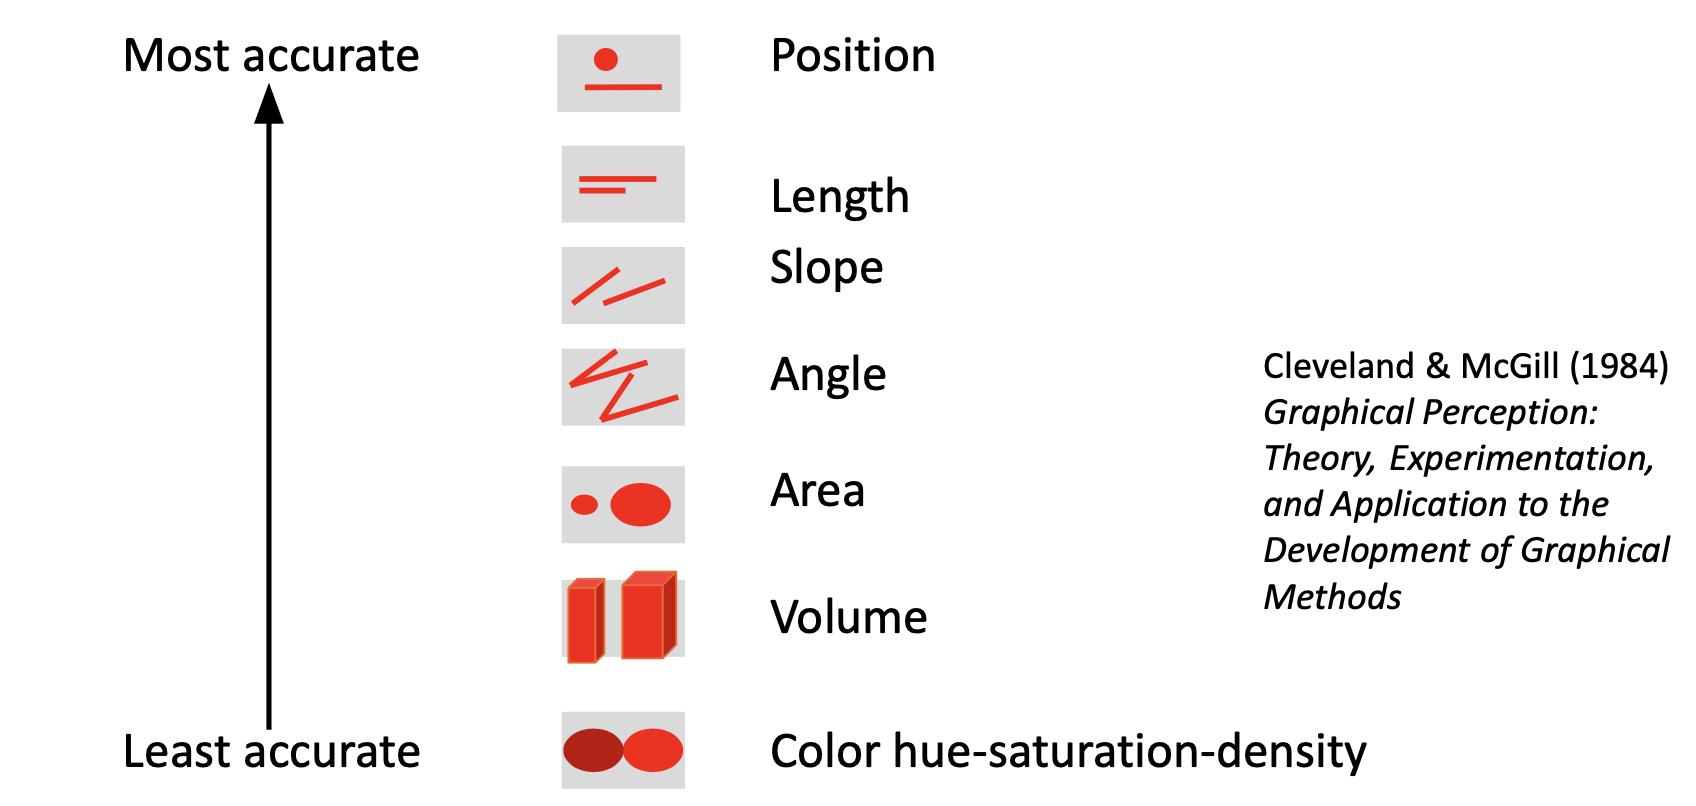
\includegraphics[width=1\textwidth]{perception-magnitudes}
    \label{fig:LABEL}
\end{figure}

\textbf{\textcolor{red}{Choose your axes wisely!}}

\textcolor{blue}{linear y-axis} vs. \textcolor{blue}{logarithmic y-axis}

\textbf{Visualizing heavy-tailed distributions}: the median is bigger than the mean. Taking the logarithmic x-axis gives a log normal distribution. This often occurs in nature. 


\section*{Heavy-tailed data: power laws}

\begin{itemize}
	\item Probability of x: $p(x) = Cx^{-a}$ 
	\begin{itemize}
		\item Very large values are rare, "but not very rare"
		\item Body size vs. city size
		\item Many natural phenomena are power laws (e.g., # of friends)
		\item For dealing with them, need to know some tricks
		\item E.g., for small $a$, mean & var =  $\infty \Rightarrow$ use median! 
		\item E.g., straight line on log-log axes: $y = Cx^{-a} \Leftrightarrow \log{y} = \log{C} - a\log{x}$
	\end{itemize}
	\item Complementary cumulative distribution function (CCDF): $P(x) := Pr\{X \geq x\}$
	\item CCDF of power law is also a power law (with exponent $\alpha - 1)$ \[
			P(x) = C \int^{\infty}_{x} x'^{-\alpha}dx' = \frac{C}{\alpha -1}x^{-(\alpha -1)}
	.\] 
\item CCDF plot is monotonically decreasing (even without binning)
\end{itemize}

% Quick centered image
\begin{figure}[H]
    \centering
    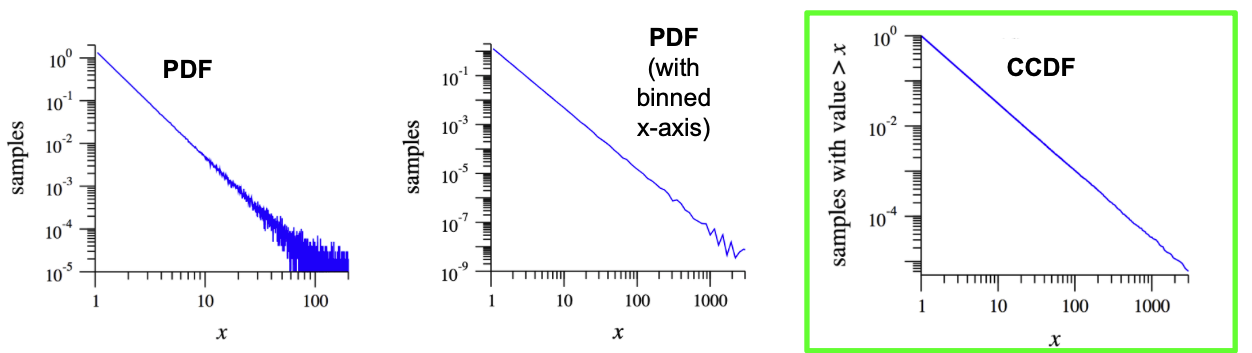
\includegraphics[width=1\textwidth]{ccdfpowerlaw}
    \label{fig:LABEL}
\end{figure}

\section*{Show data uncertainty!}

Which beer is more popular, \textbf{Guinness} or \textcolor{red}{Paulaner} ?

% Quick centered image
\begin{figure}[H]
    \centering
    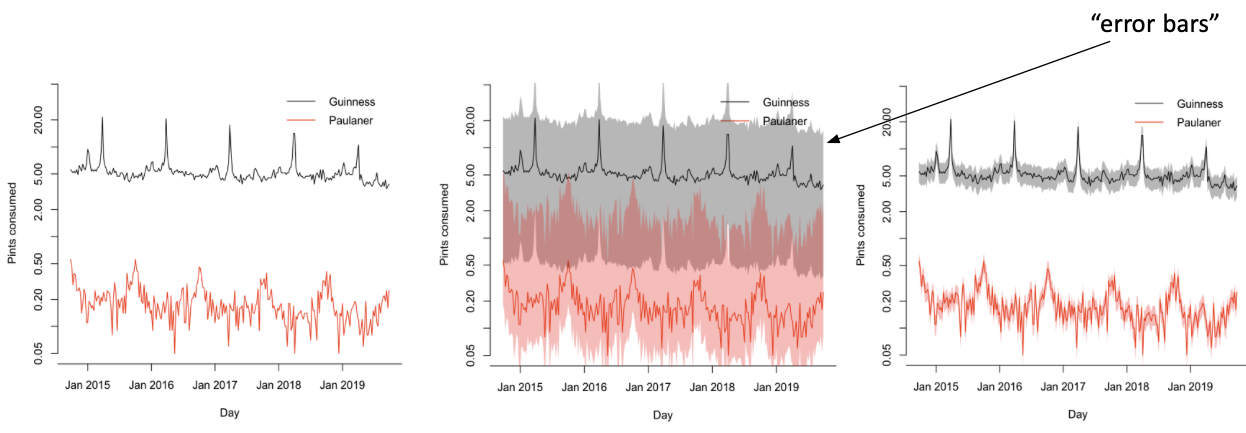
\includegraphics[width=1\textwidth]{datauncertainty}
    \label{fig:LABEL}
\end{figure}

\newpage

\section*{Use colours wisely!}

Choose colours based on the information you want to convey

% Quick centered image
\begin{figure}[H]
    \centering
    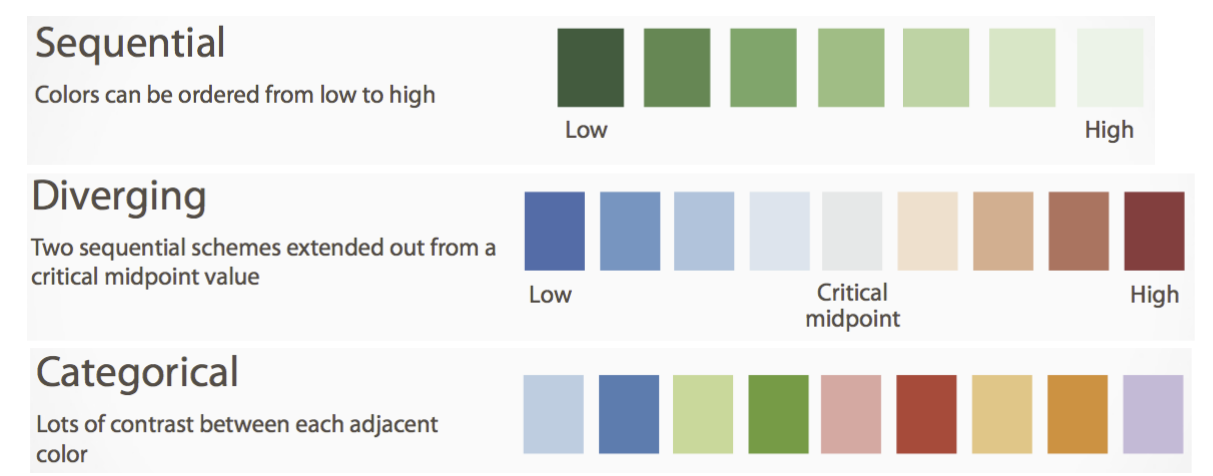
\includegraphics[width=1\textwidth]{colors}
    \label{fig:LABEL}
\end{figure}

\section*{Use visual contrast}

\begin{itemize}
	\item Use the visual contrast to highlight the important information
	\item Vary the size, shape, position, orientation, or color of an element to make the key part of the figure the most visually prominent
	\item Avoid incorporating every form of visual contrast
\end{itemize}

\section*{Part 3: a (small) selection of use cases for data visualization}

\begin{itemize}
	\item Presenting scientific results
	\item Data wrangling (multimodal data)
		\begin{itemize}
			\item Two or more distinct peaks in a histogram often \textbf{suggest 2 or more distinct populations} of samples
			\item But don't guess! Explore further by using, e.g., color and a histogram of multiple populations
		\end{itemize}
	\item Data wrangling (weird data)
		\begin{itemize}
			\item Maintain a \textbf{theory of what the data should look like}
			\item Some data is \textbf{very hard to explain}
			\item Never just blink it away! First, assume a bug. Try to fix it
			\item If not a bug: you might have made an interesting discovery!
			\item Some of science's most important findings were made by not ignoring weird data, but dwelling on it!
		\end{itemize}
	\item Journalism
\end{itemize}

\end{document}	
